%%%%%%%%%%%%%%%%%%%%%%%%%%%%%%%%%%%%%%%%%%%%%%%%%%%%%
% SUPPLEMENT FOR SWISS-SEP 2.0 DATA PREP & ANALYSIS
%%%%%%%%%%%%%%%%%%%%%%%%%%%%%%%%%%%%%%%%%%%%%%%%%%%%%

% LATEX settings
\documentclass[a4paper, notitlepage, fleqn]{article} % USE titlepage IF YOU WANT TOC TO APPEAR ON NEXT PAGE
\usepackage[a4paper]{geometry}
\usepackage{stata} 

\usepackage[T1]{fontenc}
\usepackage[utf8]{inputenc}
 
\usepackage{fullpage} % SMALL MARGINS
% \usepackage[cm]{fullpage} % VERY SMALL MARGINS
 
\usepackage{lscape} % BETTER FOR PRINTING, PAGE DISPLAYED VERTICALLY
% \usepackage{pdflscape} % BETTER FOR SCREEN, PAGE DISPLAYED HORIZONTALLY
 
\usepackage{mathtools, amssymb, bookmark, framed, longtable, booktabs, graphicx, url, multirow, cancel}
 
\usepackage{hyperref}
\hypersetup{unicode=true, pdfborder = {0 0 0}, colorlinks, citecolor=blue, filecolor=black, linkcolor=blue, urlcolor=blue, pdftitle={Swiss-SEP 2.0 supplement}, pdfauthor={Radoslaw Panczak}}

\renewcommand{\familydefault}{\sfdefault}
\usepackage[usenames, dvipsnames]{color}
\usepackage[table]{xcolor}
\usepackage[normalem]{ulem}

\usepackage[hang,flushmargin]{footmisc} 

% to avoid error http://tex.stackexchange.com/questions/165929/semiverbatim-with-tikz-in-beamer
\makeatletter
\global\let\tikz@ensure@dollar@catcode=\relax
\makeatother

\setlength{\parindent}{0pt} % no indent for ne paras
\graphicspath{ {C:/projects/SNC_Swiss-SEP2/analyses/gr} }
\setcounter{tocdepth}{2}

\usepackage{array}
\newcolumntype{L}[1]{>{\raggedright\let\newline\\\arraybackslash\hspace{0pt}}m{#1}}

% \linespread{1.3}
%
% \usepackage{setspace}
% \singlespacing
% \onehalfspacing
% \doublespacing

\usepackage{multirow}

% https://tex.stackexchange.com/questions/52317/pdftex-warning-version-allowed
\pdfminorversion=6

\title{\textbf{Swiss-SEP 2.0 index \endgraf 
Supplementary materials}}

\author{Radoslaw Panczak, Claudia Berlin, Marieke Voorpostel, Marcel Zwahlen, Matthias Egger}

\begin{document}

\maketitle
\tableofcontents
% %%%%%%%%%%%%%%%%%%%%%%%%%%%%%%%%%%%%%%%%%%%%%%%%%%%%%
% %%%%%%%%%%%%%%%%%%%%%%%%%%%%%%%%%%%%%%%%%%%%%%%%%%%%%
\newpage
\section{Data preparation}
\subsection{SNC - buildings}
% %%%%%%%%%%%%%%%%%%%%%%%%%%%%%%%%%%%%%%%%%%%%%%%%%%%%%
\subsubsection{Eligible buildings}

\textbf{Origin} buildings are defined as all buildings for which index 
is going to be calculated. These buildings need to:

\begin{enumerate}

	\item Be present at least once in the \textbf{period of 2010-2014} in the SNC dataset.
	\item Have valid 2010+ \textbf{building ID}.
	\item Have valid 2010+ \textbf{geographical coordinates}.
	\item Belong to category of 'normal' \textbf{residential buildings} (ie. no prisons, churches or nursing homes; see Appendix).
	
\end{enumerate}
	
Buildings are selected from the \texttt{snc2\_std\_pers\_90\_00\_14\_all\_206\_full} dataset 
and processed as follows:
	
\begin{enumerate}

	\item All buildings that have an ID and coordinates on any year from \textbf{2010} onward are selected
		
	\item Submeter coordinates are rounded to 1m
		
	\item \textbf{Newest} coordinates are always used when several are available under the same building ID
	
	\item \textbf{Non-residential} buildings (see above) are excluded
	
	\item Buildings having different ID but \textbf{same cordinates} are groupped together using synthetic 'GIS ID'
		(for instance 153 (sic!) different buidling IDs pointing to the same coordinates \href{https://goo.gl/maps/eC8fDZtEboP2}{on a caravan site?})
		
\end{enumerate}

These coordinates become \textbf{n'hood centres} for network analysis and construction of an index.  

% %%%%%%%%%%%%%%%%%%%%%%%%%%%%%%%%%%%%%%%%%%%%%%%%%%%%%
\subsubsection{Results}

Distribution of years from which coordinates of a building are taken: 
\begin{stlog}\input{log/ol_2.log.tex}\end{stlog}
Note the distinction between IDs (ie. small amount of buildings with different ID but same coordinates):
\begin{stlog}\input{log/ol_3.log.tex}\end{stlog}
% %%%%%%%%%%%%%%%%%%%%%%%%%%%%%%%%%%%%%%%%%%%%%%%%%%%%%
% %%%%%%%%%%%%%%%%%%%%%%%%%%%%%%%%%%%%%%%%%%%%%%%%%%%%%
\newpage
\subsection{SE}

% %%%%%%%%%%%%%%%%%%%%%%%%%%%%%%%%%%%%%%%%%%%%%%%%%%%%%
\subsubsection{Eligible persons \& households}

\textbf{Destination} households are defined as all household that can provide information for calculation of the index. 
They need to be present in at least one Structural Survey (SE) during the period of 2012-2015.
Surveys of 2010 and 2011 do not provide information
about m2 area of the flat which is needed for calculation of standardised rent and were therefore excluded. 
Additionally, there are some reservations as to quality of the 2010 data. \\

In order to be included, SE personal record must (sequentially): 

\begin{enumerate}

	\item Link to household record.
	
	\item Link to full SNC for \texttt{buildid}.\footnote{Apart from 2015 SE data that are not yet included in the full SNC; \texttt{egid} identifier of the building was kindly provided by the SNC team}
	
	\item Link to valid coordinates (from ORIGINS dataset, see previous section).

\end{enumerate}

Key variables\footnote{Where 'yy' in the name stands for the year of the SE} needed are then selected from each of the sources:
	
\begin{enumerate}

	\item \texttt{sncid, hhyid, age, sex, educ\_agg, educ\_curr, occup\_isco, workstatus} from the 
		\texttt{SEyy\_pers\_full} dataset.
		
	\item \texttt{hhyid, hhtype, hhpos, hhpers, flatrooms, typeowner, rentnet}
		from the \texttt{SEyy\_hh\_full} dataset (linked via \texttt{hhyid}) 
	
	\item \texttt{buildid}
		from the \texttt{snc2\_std\_pers\_90\_00\_14\_all\_206\_full} dataset 
		(linked via \texttt{sncid})
	
	\item \texttt{geox, geoy}
		from the \texttt{ORIGINS} dataset (linked via \texttt{buildid} 	)

\end{enumerate}

At next stage, individuals are excluded if:

\begin{enumerate}
	
	\item Are younger than 19 at the time of SE.
	
	\item Have one of the 'unusual' types of residence permit 
	(Cross-border commuter (G), Short stay (L), Asylum seeker (N), People in need of protection (S), 
	Person required to notify (Meldepflichtige), 
	Diplomat/internat. official with diplomatic immunity, 
	Internat. official without diplomatic immunity, 
	Not classified elsewhere)	
	
	\item If individual participated in more than one SE, the latest record is kept.

\end{enumerate}

For remaining individuals and their households, the following data are prepared:

\begin{enumerate}
	
	\item Individuals are flagged if they work in \textbf{manual or unskilled occupations} 
		(BUT only if they are in \textbf{paid employment} at the time of SE; see below).
	\item Individuals are flagged if they have \textbf{no formal or have only compulsory education} 
		AND are not currently pursuing any further education.
	\item Households have their \textbf{crowding} (number of persons per room) calculated.
	\item Households are flagged if they have \textbf{three to five rooms and are rented}.
	
\end{enumerate}

% %%%%%%%%%%%%%%%%%%%%%%%%%%%%%%%%%%%%%%%%%%%%%%%%%%%%%
\newpage
\subsubsection{Exclusions: eligibility criteria}

\begin{table}[!htbp]
\centering
%\caption{My caption}
%\label{my-label}
\begin{tabular}{rrrrr}
\hline
\multicolumn{1}{l}{\multirow{2}{*}{Exclusion}} & \multicolumn{4}{c}{Year}                                                                                  \\
\multicolumn{1}{l}{}                           & \multicolumn{1}{c}{2012} & \multicolumn{1}{c}{2013} & \multicolumn{1}{c}{2014} & \multicolumn{1}{c}{2015} \\
\hline
\multicolumn{1}{l}{\textbf{Start}}             & 270654               & 266803               & 272966               & 255969               \\
\quad Age \textless 19				           & 14791                 & 14463                 & 14184                 & 12929                 \\
\quad Permit      					           & 570                 & 724                 & 692                 & 611                 \\
\quad No household link				           & 41319                 & 40275                 & 42175                 & 35900                 \\
\quad No building ID 					       & 38                 & 7                 & 4                 & 0                 \\
\quad Excluded building 				       & 1334                 & 1297                 & 1410                 & 3965                 \\
\hline
\multicolumn{1}{l}{\textbf{End}}               & 227963                 & 225224                 & 229377                 & 216104                 \\
\hline
\end{tabular}
\end{table}

The explanation of substantial amount of individuals not linked to households came from BfS: \\

\emph{The reference person has to fill out a form for all household members. As the FSO "calibrate" the structural survey using the information from STATPOP they decided to not include the information for the additional household members if the household structure (number of hh members, gender information) given on the SE household form didn’t match the household information in STATPOP. This always applies for around 14\% of the SE reference persons.} \\ 

\subsubsection{Exclusions: multiple SE}

In cases when one person participated in more than one SE only newer records were kept.  
\begin{stlog}\input{log/ol_6.log.tex}\end{stlog}
% %%%%%%%%%%%%%%%%%%%%%%%%%%%%%%%%%%%%%%%%%%%%%%%%%%%%%
\subsubsection{Results}
Distribution of SE individuals over years:
\begin{stlog}\input{log/ol_7.log.tex}\end{stlog}
Note the distinction between individuals, households, buildings and \texttt{gisid}, ie. individual and two spatial resolutions:
\begin{stlog}\input{log/ol_8.log.tex}\end{stlog}
% %%%%%%%%%%%%%%%%%%%%%%%%%%%%%%%%%%%%%%%%%%%%%%%%%%%%%
\subsubsection{Limitations}

\begin{enumerate}

	\item Major limitation is that, compared to SEP 1.0, there is no way to define \textbf{head of the household} - 
		all respondents (see exclusions) of the SE are then used, irrespectively of their position in household.
		
	\item 2014 SE dataset is \textbf{missing information on \textit{'Sozioprofessionelle Kategorie'}} (variable \texttt{sopc}).  
		It has been also signalled by BfS that this variable was of poor quality in 2010-2013 years. 
		Therefore, it is not possible to identify individuals in manual and unskilled occupations in the same way as during 
		construction of original index. That was mitigated by using the 
		\href{http://www.ilo.org/public/english/bureau/stat/isco/isco08/index.htm}{\textbf{ISCO-08 codes}} of occupations 
		to define manual and unskilled workers and farmers.
		Individuals whose occupations belong to one of the major groups 7, 8 \& 9 (for manual and unskilled) and 6 (farmers) were selected.\footnote{Additionally, 
		sensitivity analyses were done with more strict selection of ISCO codes (major groups 8 \& 9 only) as well as 	
		by converting ISCO-08 codes to \href{http://www.harryganzeboom.nl/isco08/qa-isei-08.htm}{\textbf{ISEI-08 codes}} 
		to obtain continuous measure of 'International Socio-Economic Index of occupational status'and calculating summary of these vlaues in n'hood} 				
		Note that occupation codes are available only for people in \textbf{paid employment} so the denominator 
		for calculating 'employment' domain was adapted and all individuals that were not in paid employment were excluded.	
		Also - small proportion of people eligible for calculations based on ISCO codes had them missing. Again, they were included in the study
		but had their profession information replaced to missing and again the denominator was adjusted to reflect that.
		
	\item There is significant amount of individuals in SE data with \textbf{no link to household SE file} and all these records were excluded. 
	
\end{enumerate}
% %%%%%%%%%%%%%%%%%%%%%%%%%%%%%%%%%%%%%%%%%%%%%%%%%%%%%
% %%%%%%%%%%%%%%%%%%%%%%%%%%%%%%%%%%%%%%%%%%%%%%%%%%%%%
\newpage
\subsection{Road network}

% %%%%%%%%%%%%%%%%%%%%%%%%%%%%%%%%%%%%%%%%%%%%%%%%%%%%%
\subsection{Setup}

\begin{enumerate}

	\item Network analyses were done using updated version of \textbf{swissTLM3D} data 
		(1.5 version as compared to 1.0 vesrsion in the previous edition).
	
	\item Network analyses were done using ArcGIS 10.5 (previously - ArcGIS 10.2).
	
	\item Network analyses took all SNC buildings as \texttt{ORIGINS} and calculated 
		50 closest \texttt{DESTINATIONS} from the SE dataset.
		\footnote{In that logic, the n'hood is either constructed from one SE household and 49 SE neighbours 
		OR 50 SE neighbours if the n'hood centre is not the SE household}		
	
	\item Treshold for n'hood construction was set up to be maximum 20 km (measured along the road network).\footnote{That was based 
		on preliminary checks with data, results of previous analyses \& common sense rationale (hard to say it's n'hood if households are more than 20km apart\ldots}
	
	\item As in the 1.0 index, separate n'hoods were created using rented, 3-5 bedroom flats as \texttt{DESTINATIONS}. 

\end{enumerate}

Schematic representation of n'hood 'search' comparing the use of all buildings to use of sample buildings could be visualized as follows: 

\begin{center}
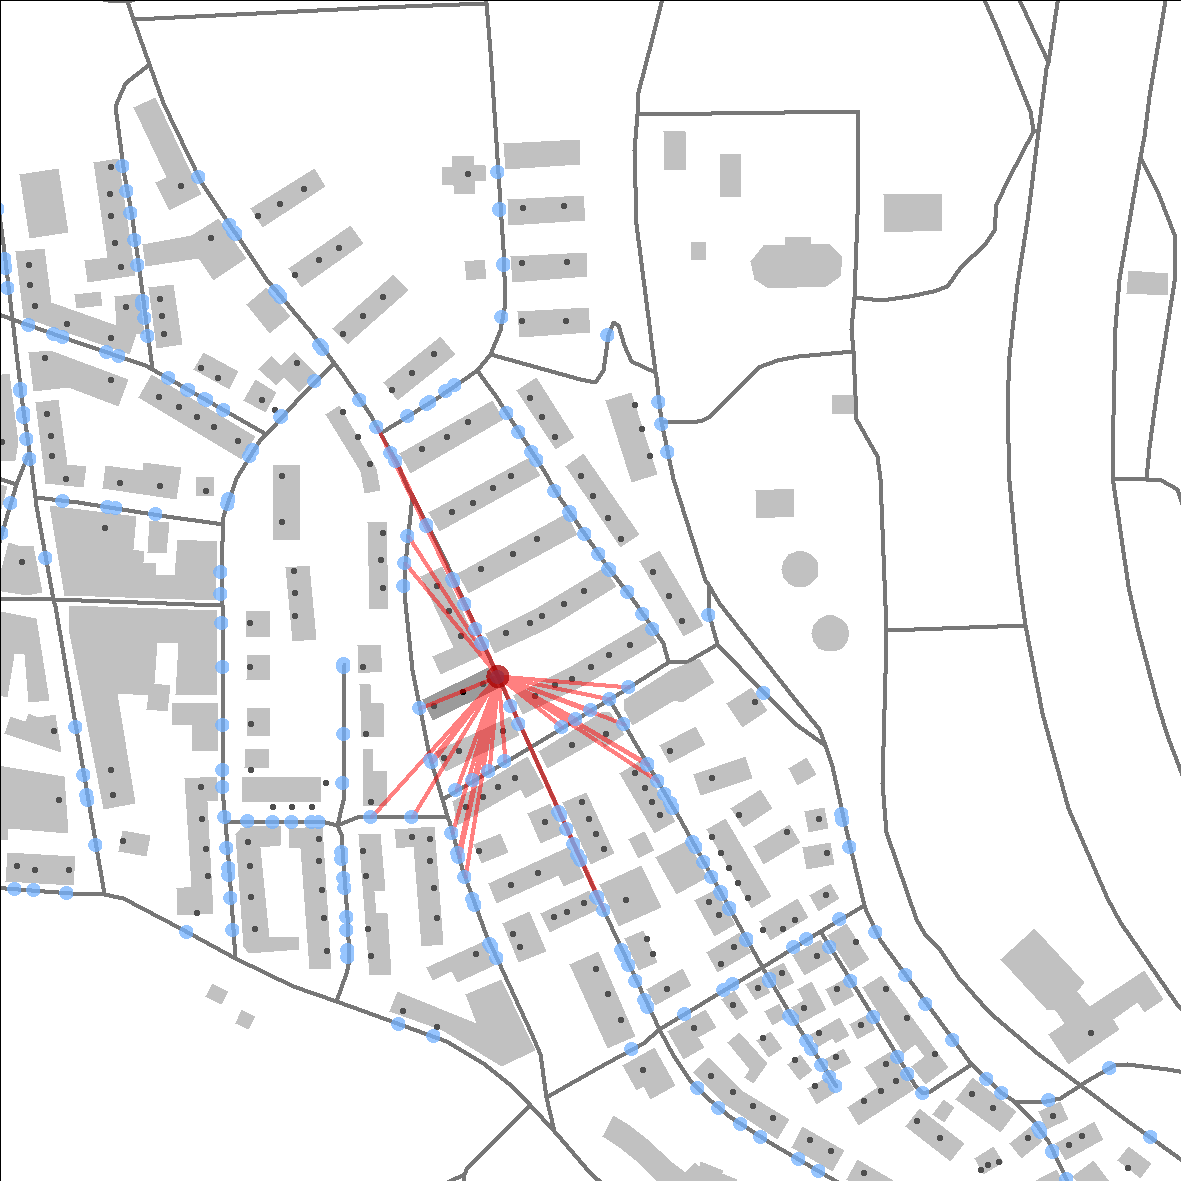
\includegraphics[width=.45\textwidth]{gr-ext/all.png}
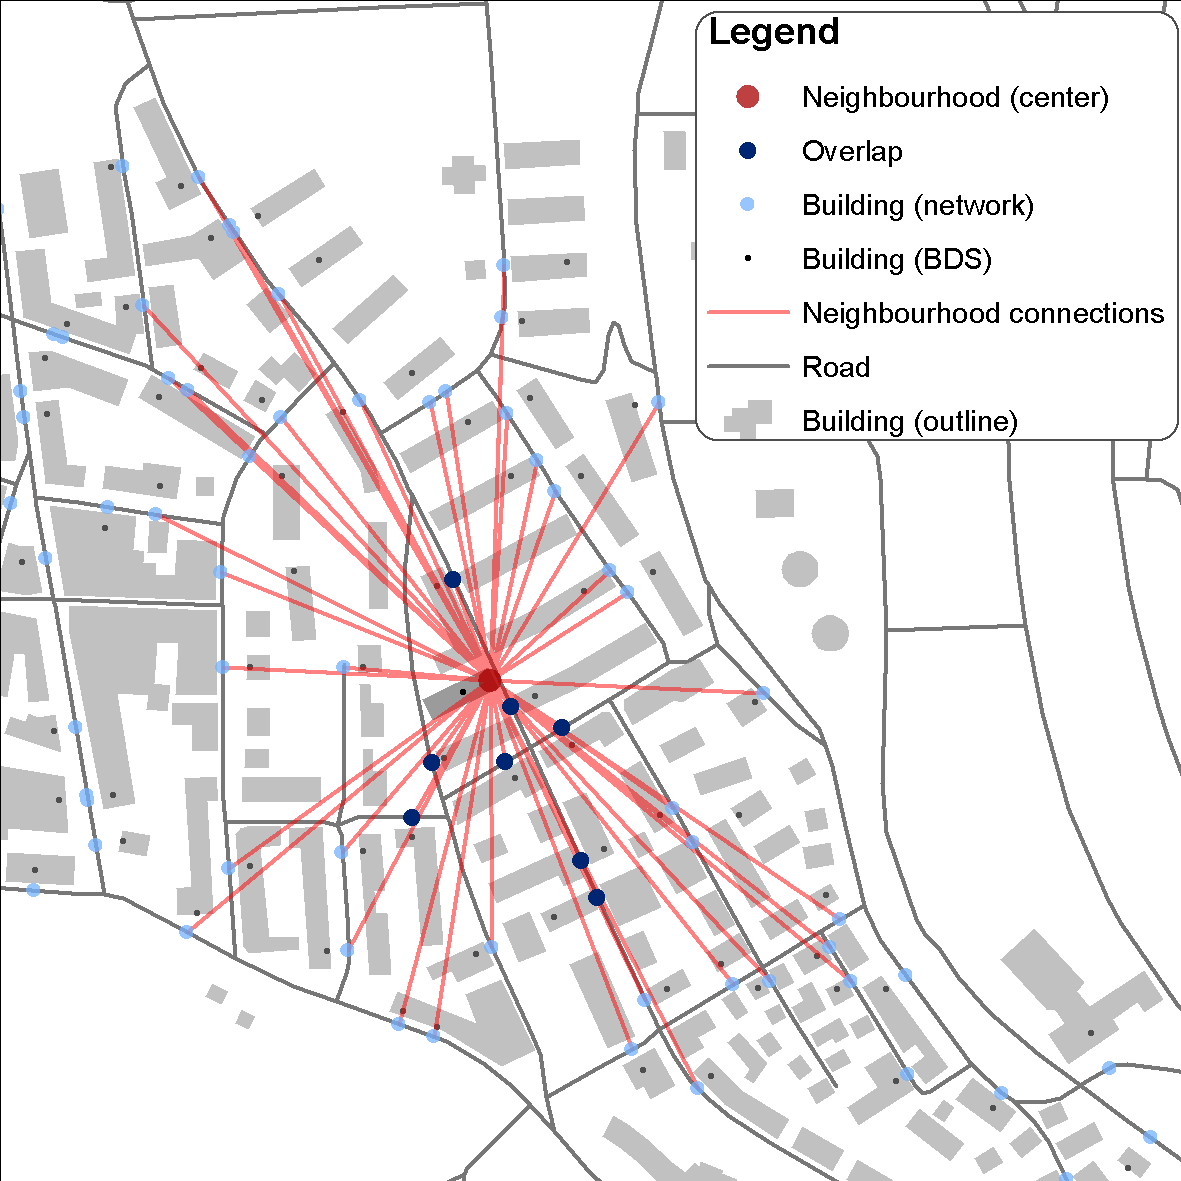
\includegraphics[width=.45\textwidth]{gr-ext/sample.png} 
\end{center}

Small \textit{ad hoc} corrections of the \textbf{swissTLM3D} dataset were necessary in cases where unconnected segments of the road network were found. These features were then removed: 

\begin{center}
\includegraphics[width=.5\textwidth]{gr-ext/nw_edits_4.png}
\end{center}

% %%%%%%%%%%%%%%%%%%%%%%%%%%%%%%%%%%%%%%%%%%%%%%%%%%%%%
\subsubsection{Results - buildings}

Vast majority of the SNC buildings (\texttt{ORIGINS}) have network connections to 50 SE buildings (\texttt{DESTINATIONS})
\footnote{Keep in mind this results will get even better when we move from buildings to households}: 
\begin{stlog}\input{log/ol_12.log.tex}\end{stlog}
The two cases of buildings with no neighbours are legitimate and really have no neighbours on the (highway restricted) road network: 
	one of the buildings is located on \href{https://goo.gl/maps/L5sLmrMXZap}{Ufenau Island}, Lake Zurich; 
	and the other - right next to highway,  \href{https://goo.gl/maps/fxPCBS5TmEQ2}{on the shore of Thunersee}. 
	These two buildings were excluded from the analyses and have no index. \\
	
\begin{center}
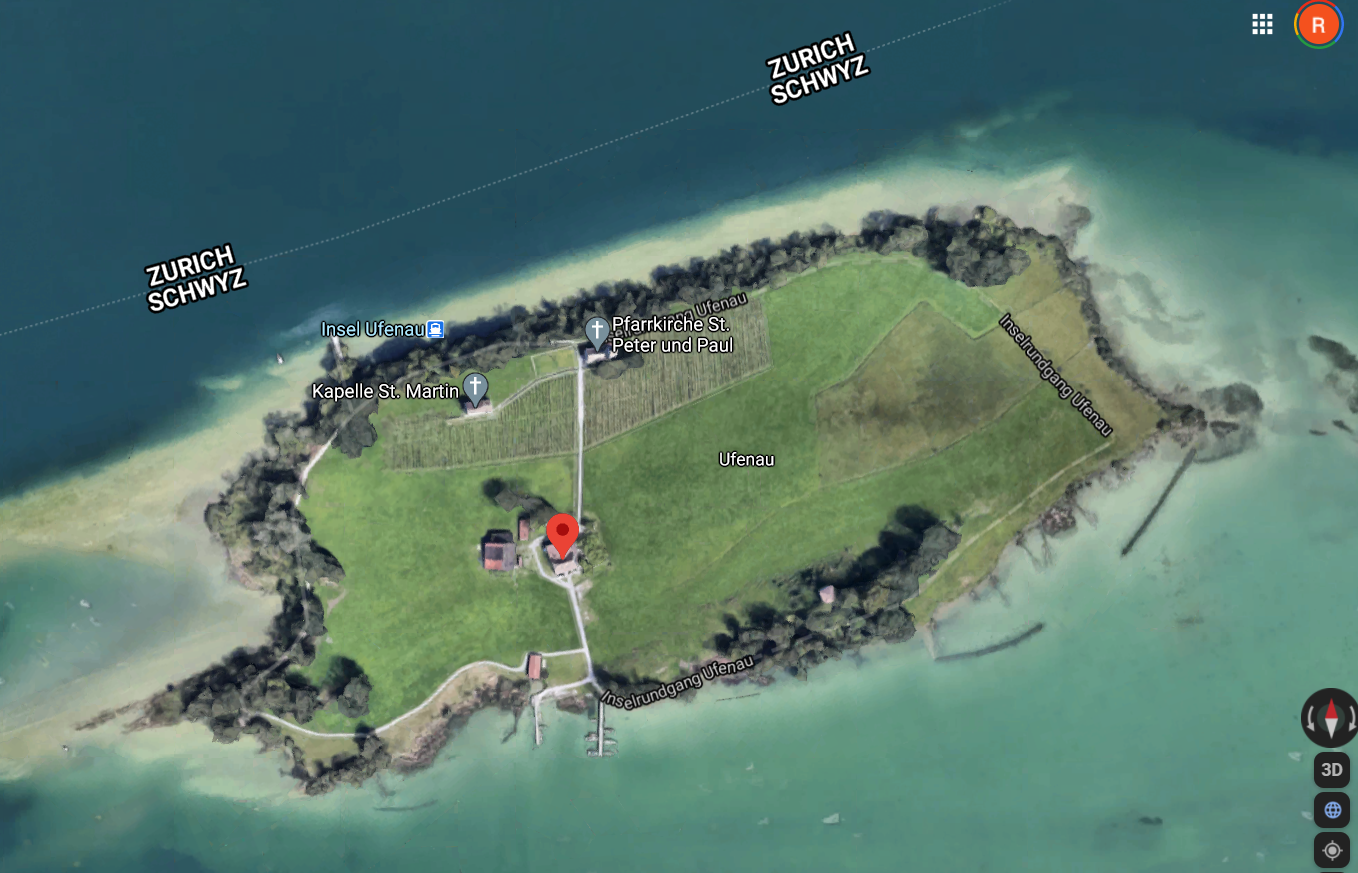
\includegraphics[width=.6\textwidth]{gr-ext/ufenau.png} 
\end{center}

Similarly, buildings with n'hoods not meeting the 50 households treshold size will be flagged. \\

Few areas where less than 50 buildings were found in the n'hood (respecting 20km road network distance) were located in sparesly populated areas such as:
	\href{https://goo.gl/maps/BXbgyCYtuGU2}{Gondo} (close to Simplon Pass) or \href{https://goo.gl/maps/mg15ptJPVTJ2}{Avers} (Grisons) villages. \\

Building with the biggest (89!) number of SE households is located in \href{https://goo.gl/maps/oFeag8mQFdS2}{Lausanne} and is in fact pretty big.
% %%%%%%%%%%%%%%%%%%%%%%%%%%%%%%%%%%%%%%%%%%%%%%%%%%%%%
\subsubsection{Results - households}

The n'hood structure of connectivity between SNC buildings \& SE households changes (for better! ;)
when we move from buildings to households. 
Keep in mind - there might be more than one SE household in a certain building and if we take that into account 
household n'hoods can get smaller than building n'hoods. 
Number of buildings (within 20km):
\begin{stlog}\input{log/ol_14.log.tex}\end{stlog}
Number of households (within 20km):
\begin{stlog}\input{log/ol_15.log.tex}\end{stlog}
Number of individuals:
\begin{stlog}\input{log/ol_16.log.tex}\end{stlog}
Average distance [in meters] to the building where furthest SE household is located (within 20km):
\begin{stlog}\input{log/ol_17.log.tex}\end{stlog}
% %%%%%%%%%%%%%%%%%%%%%%%%%%%%%%%%%%%%%%%%%%%%%%%%%%%%%
\subsubsection{Results - households, rent}

As expected, results are slightly worse when we limit network analyses to 3-5 bedroom rented flats only. \\
\\
Number of rented buildings (within 20km):
\begin{stlog}\input{log/ol_20.log.tex}\end{stlog}
Number of rented households (within 20km):
\begin{stlog}\input{log/ol_21.log.tex}\end{stlog}
Average distance [in meters] to the building where furthest rented SE household is located (within 20km):
\begin{stlog}\input{log/ol_22.log.tex}\end{stlog}
% %%%%%%%%%%%%%%%%%%%%%%%%%%%%%%%%%%%%%%%%%%%%%%%%%%%%%
% %%%%%%%%%%%%%%%%%%%%%%%%%%%%%%%%%%%%%%%%%%%%%%%%%%%%%
\newpage
\subsection{Swiss Household Panel}

% %%%%%%%%%%%%%%%%%%%%%%%%%%%%%%%%%%%%%%%%%%%%%%%%%%%%%
\subsubsection{Setup}

Combined samples I, II and III of the Swiss Household Panel (SHP) dataset were used to validate the index

\begin{enumerate}

	\item SHP households were included if: 

	\begin{enumerate}	
		\item they provided questionnaire in 2014 
		\item had complete information regarding the address
		\item address was successfully geocoded\footnote{Geocoding was done using map.geo.admin.ch service.}
	\end{enumerate}	
		
	\item Same variables that were used in Table 2 of original publication are extracted
		\footnote{Note that 'Savings min. 500 SFrs monthly' has changed - it used to refer to '100 CHF'}	
		
	\item Each geocoded household was spatially linked to the closest building from the ORIGINS dataset 
\end{enumerate}
% %%%%%%%%%%%%%%%%%%%%%%%%%%%%%%%%%%%%%%%%%%%%%%%%%%%%%
\subsubsection{Variables}
\begin{stlog}\input{log/ol_24.log.tex}\end{stlog}
% %%%%%%%%%%%%%%%%%%%%%%%%%%%%%%%%%%%%%%%%%%%%%%%%%%%%%
\subsubsection{Geocoding status across surveys}
\begin{stlog}\input{log/ol_25.log.tex}\end{stlog}
% %%%%%%%%%%%%%%%%%%%%%%%%%%%%%%%%%%%%%%%%%%%%%%%%%%%%%
% %%%%%%%%%%%%%%%%%%%%%%%%%%%%%%%%%%%%%%%%%%%%%%%%%%%%%
\newpage
\subsection{SNC - mortality}

% %%%%%%%%%%%%%%%%%%%%%%%%%%%%%%%%%%%%%%%%%%%%%%%%%%%%%
\subsubsection{Setup}

Association of Swiss-SEP with mortality will be assessed using two models based on complete SNC: 
'age \& sex' and 'semi adjusted'  
(additionally taking into account: nationality, civil status, language region \& level of urbanization). Setup for the analyses in this scenario: 
\begin{enumerate}

	\item Individuals who are recorded in (at least one of the) 2012 - 2018 Censuses are included
	\item Individuals below age 30 on the 1.1.2012 are excluded
	\item Date of entry is either 1.1.2012 or earliest census if individual was not recorderd in 2012
	\item Individuals who died on or before 12.31.2011 are excluded (unless the death was cancelled in the dataset)
	\item For individuals having information on one of the covariates recorded inseveral censuses the latest one is used
	\item Individuals with missing civil status were excluded
	\item Rhaeto-Romansch language region was merged to German
	\item Individuals with no link to the index were excluded
	
\end{enumerate}

% %%%%%%%%%%%%%%%%%%%%%%%%%%%%%%%%%%%%%%%%%%%%%%%%%%%%%
\subsubsection{Individuals \& deaths included}
\begin{stlog}\input{log/ol_27.log.tex}\end{stlog}
% %%%%%%%%%%%%%%%%%%%%%%%%%%%%%%%%%%%%%%%%%%%%%%%%%%%%%
\subsubsection{Causes of deaths}
\begin{stlog}\input{log/ol_28.log.tex}\end{stlog}
% %%%%%%%%%%%%%%%%%%%%%%%%%%%%%%%%%%%%%%%%%%%%%%%%%%%%%
\subsubsection{Variables}
\begin{stlog}\input{log/ol_29.log.tex}\end{stlog}
% %%%%%%%%%%%%%%%%%%%%%%%%%%%%%%%%%%%%%%%%%%%%%%%%%%%%%
\subsubsection{Last census seen}
\begin{stlog}\input{log/ol_30.log.tex}\end{stlog}
% %%%%%%%%%%%%%%%%%%%%%%%%%%%%%%%%%%%%%%%%%%%%%%%%%%%%%
\newpage
\section{Data analysis}
\subsection{PCA on n'hood aggregated characteristics}
\begin{stlog}\input{log/ol_32.log.tex}\end{stlog}
% %%%%%%%%%%%%%%%%%%%%%%%%%%%%%%%%%%%%%%%%%%%%%%%%%%%%%
\newpage
\subsection{Building construction period}

Construction period of the building is retrived sfrom \texttt{STATPOP 2018} dataset. Detailed typology is recoded to binary indicator flagging buildings constructed on or after 2001. Buidlings with missing information about age are treated as 'old' ones. 

In case of small onount of buildings with same gisid but different buildid 
(spatial duplicates, n = 1886, 0.1\%) 
when two different periods were recorded (old AND new) building is treated as new. 
\begin{stlog}\input{log/ol_35.log.tex}\end{stlog}
% %%%%%%%%%%%%%%%%%%%%%%%%%%%%%%%%%%%%%%%%%%%%%%%%%%%%%
\newpage
\subsection{Hybrid version of SEP}

This solution is mixing versions 1.0 \& 2.0. First the new buildings have value of index 1.0 assigned using the closest (linear dstance) neighbour. 

Then, construction period of the building is retrived sfrom \texttt{STATPOP 2018} dataset and then buildings built before year 2000 have the values of 1.0 index assigned and buildings constructed after 2000 have new values assigned. Buildings without the defined period of construction keep values 1.0 also. 
% %%%%%%%%%%%%%%%%%%%%%%%%%%%%%%%%%%%%%%%%%%%%%%%%%%%%%
\subsection{Index deciles}
\begin{stlog}\input{log/ol_37.log.tex}\end{stlog}
% %%%%%%%%%%%%%%%%%%%%%%%%%%%%%%%%%%%%%%%%%%%%%%%%%%%%%
\subsection{Quantiles}

Note that the deciles of third version in \texttt{user} dataset:
\begin{stlog}\input{log/ol_38.log.tex}\end{stlog}
... are tad 'broken' in \texttt{snc} dataset :
\begin{stlog}\input{log/ol_39.log.tex}\end{stlog}
... This is expected behaviour since SNC dataset includes buildings with different BfS IDs but same coordinates. 
Same applies for missing data - there are few buildings where SEP could not have been calculated due to road network constraints.  
\begin{landscape}
Some transitions happened:  
\begin{stlog}\input{log/ol_40.log.tex}\end{stlog}
\end{landscape}

% %%%%%%%%%%%%%%%%%%%%%%%%%%%%%%%%%%%%%%%%%%%%%%%%%%%%%
\subsection{Bland Altman plots of diffs}
\subsubsection{SEP2 vs. SEP1}

\begin{center}
\includegraphics[width=\textwidth]{gr/BA_sep1_sep2.png} 
\end{center}

\subsubsection{SEP3 vs. SEP1}

\begin{center}
\includegraphics[width=\textwidth]{gr/BA_sep1_sep3.png} 
\end{center}
% %%%%%%%%%%%%%%%%%%%%%%%%%%%%%%%%%%%%%%%%%%%%%%%%%%%%%
\newpage
\subsection{Tables}
\newpage
\subsubsection{Old index}
\begin{landscape}
\begin{footnotesize}
\input(table-1)
\end{footnotesize}
\end{landscape}

\newpage
\subsubsection{New index}
\begin{landscape}
\begin{footnotesize}
\input(table-2)
\end{footnotesize}
\end{landscape}

\newpage
\subsubsection{Hybrid index}
\begin{landscape}
\begin{footnotesize}
\input(table-3)
\end{footnotesize}
\end{landscape}

% %%%%%%%%%%%%%%%%%%%%%%%%%%%%%%%%%%%%%%%%%%%%%%%%%%%%%
\newpage
\subsection{Maps}
\subsubsection{Original map}
\begin{center}
\includegraphics[width=\textwidth]{gr/sep-old.png} 
\end{center}
\newpage 
\subsubsection{SEP 2 \& 3 index}

Using hexagonal grid 500m size.  
\begin{center}
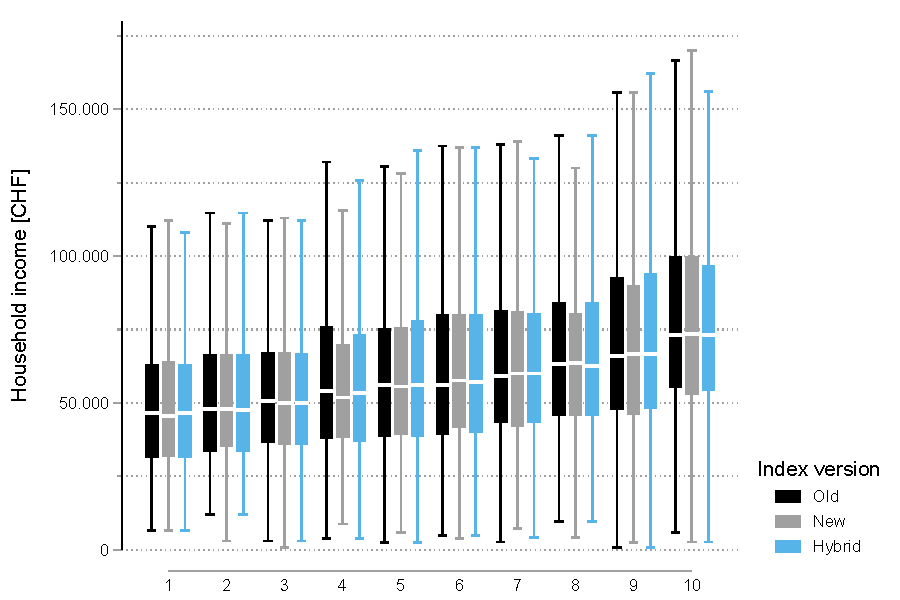
\includegraphics[width=\textwidth]{C:/projects/SNC_Swiss-SEP2/analyses/Figure_1.png} 
\end{center}
\newpage
\subsubsection{Differences}
\begin{center}
\includegraphics[width=\textwidth]{C:/projects/SNC_Swiss-SEP2/carto/08_sep-diff-grid_hex_500.png} 
\end{center}
% %%%%%%%%%%%%%%%%%%%%%%%%%%%%%%%%%%%%%%%%%%%%%%%%%%%%%
% %%%%%%%%%%%%%%%%%%%%%%%%%%%%%%%%%%%%%%%%%%%%%%%%%%%%%
\newpage
\subsection{Validation - SHP data}

% %%%%%%%%%%%%%%%%%%%%%%%%%%%%%%%%%%%%%%%%%%%%%%%%%%%%%
\subsubsection{Income graph - original}

\begin{center}
\includegraphics[width=.75\textwidth]{gr-orig/orig_income.png} 
\end{center}

% %%%%%%%%%%%%%%%%%%%%%%%%%%%%%%%%%%%%%%%%%%%%%%%%%%%%%
\subsubsection{Income graph - new indices}
\begin{center}
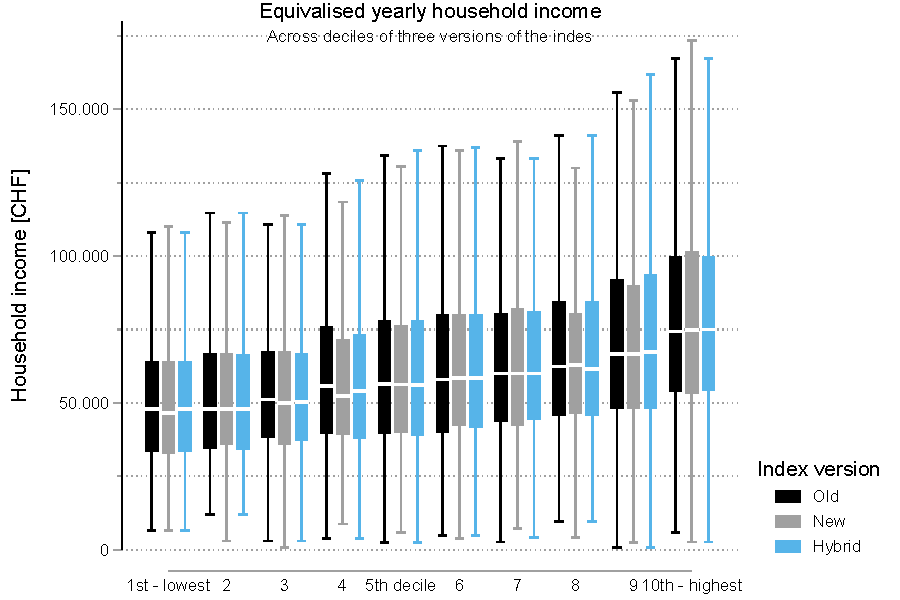
\includegraphics[width=.75\textwidth]{gr/shp_income.pdf} 
\end{center}

\newpage
\begin{center}
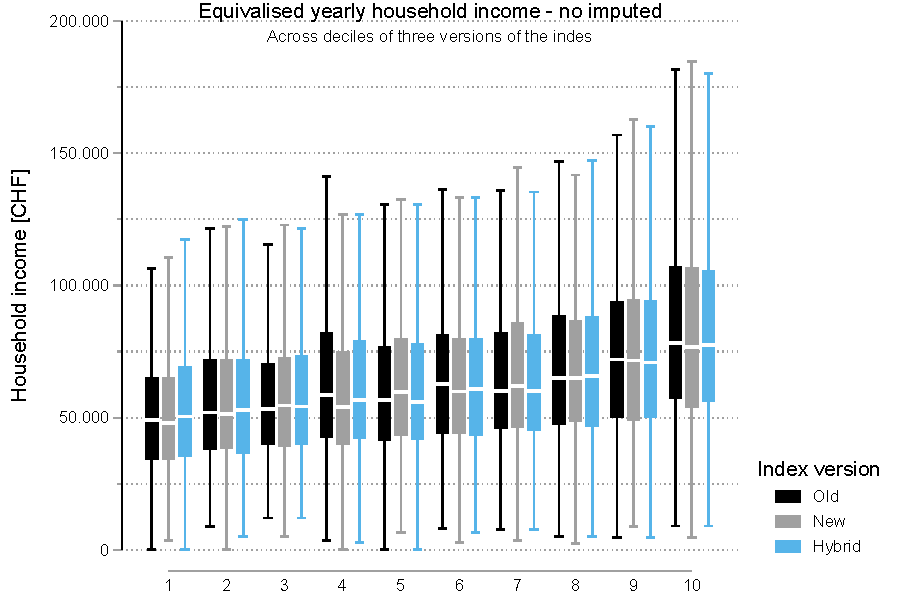
\includegraphics[width=.75\textwidth]{gr/shp_income_imp.pdf} 
\end{center}

% %%%%%%%%%%%%%%%%%%%%%%%%%%%%%%%%%%%%%%%%%%%%%%%%%%%%%
\newpage
\subsubsection{Financial variables table - original}

\begin{center}
\includegraphics[width=.95\textwidth]{gr-orig/orig_shp_table.png} 
\end{center}

% %%%%%%%%%%%%%%%%%%%%%%%%%%%%%%%%%%%%%%%%%%%%%%%%%%%%%
\newpage
\subsubsection{Financial variables table - 1.0}
\begin{stlog}\input{log/ol_43.log.tex}\end{stlog}
\newpage
\begin{stlog}\input{log/ol_44.log.tex}\end{stlog}
\newpage
\begin{stlog}\input{log/ol_45.log.tex}\end{stlog}
% %%%%%%%%%%%%%%%%%%%%%%%%%%%%%%%%%%%%%%%%%%%%%%%%%%%%%
\newpage
\subsubsection{Financial variables table - 2.0}
\begin{stlog}\input{log/ol_46.log.tex}\end{stlog}
\newpage
\begin{stlog}\input{log/ol_47.log.tex}\end{stlog}
\newpage
\begin{stlog}\input{log/ol_48.log.tex}\end{stlog}
% %%%%%%%%%%%%%%%%%%%%%%%%%%%%%%%%%%%%%%%%%%%%%%%%%%%%%
\newpage
\subsubsection{Financial variables table - 3.0}
\begin{stlog}\input{log/ol_49.log.tex}\end{stlog}
\newpage
\begin{stlog}\input{log/ol_50.log.tex}\end{stlog}
\newpage
\begin{stlog}\input{log/ol_51.log.tex}\end{stlog}
% %%%%%%%%%%%%%%%%%%%%%%%%%%%%%%%%%%%%%%%%%%%%%%%%%%%%%
\newpage
\subsection{Validation - SNC mortality}

\subsubsection{All cause mortality - original}

\begin{center}
\includegraphics[width=.50\textwidth, angle = 270]{gr-orig/orig_hr_all.png} 
\end{center}

Note: 	Calculations from 'old' SNC data from the \textbf{2001 - 2008 period}, as described in original paper!

% %%%%%%%%%%%%%%%%%%%%%%%%%%%%%%%%%%%%%%%%%%%%%%%%%%%%%
\subsubsection{All cause mortality - new indices}
\begin{center}
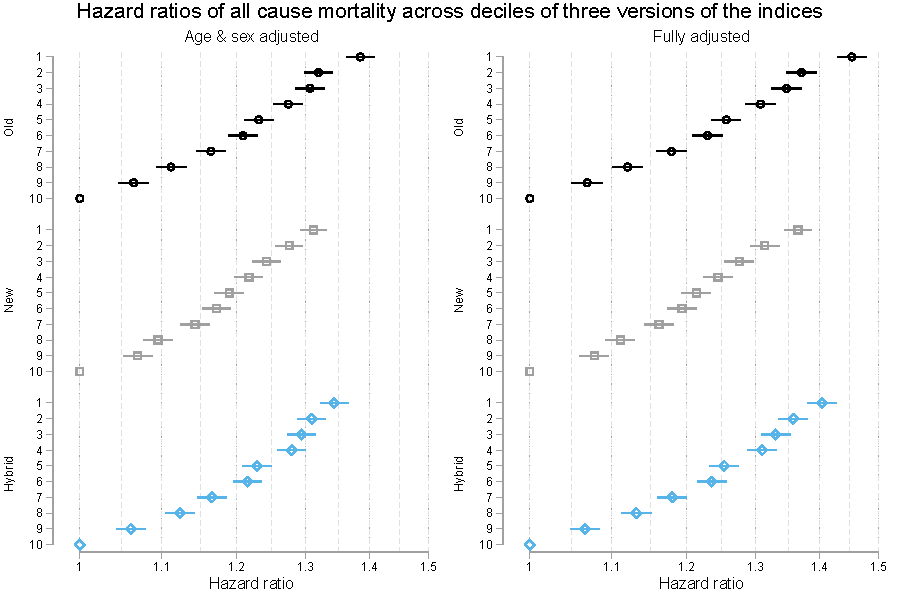
\includegraphics[width=\textwidth]{gr/sep3.pdf}
\end{center}

Note: 	Results from Cox models. Calculations from 'new' SNC data from the \textbf{2012 - 2018 period}!  
		'Age \& sex' - adjusted for age (via \texttt{stset}) and sex (as in original figure above);  
		'Adjusted' - additionally adjusted for civil status, nationality, level of urbanization and language region.  
		This is not the same adjustment as in adsjudsted models in original papers since we are missing some crucial variables. 
% %%%%%%%%%%%%%%%%%%%%%%%%%%%%%%%%%%%%%%%%%%%%%%%%%%%%%
\newpage
\subsubsection{Cause specific mortality - original}

\begin{center}
\includegraphics[width=.60\textwidth]{gr-orig/orig_hr_spec.png} 
\end{center}

% %%%%%%%%%%%%%%%%%%%%%%%%%%%%%%%%%%%%%%%%%%%%%%%%%%%%%
\newpage
\subsubsection{Cause specific mortality - 1.0}
\begin{stlog}\input{log/ol_54.log.tex}\end{stlog}
Note for both tables: HRs for the 10th (lowest SEP) decile compared to 1st (highest SEP). 
Breast and prostate cancer: for men and women respectively. 

% %%%%%%%%%%%%%%%%%%%%%%%%%%%%%%%%%%%%%%%%%%%%%%%%%%%%%
\newpage
\subsubsection{Cause specific mortality - 2.0 results}
\begin{stlog}\input{log/ol_56.log.tex}\end{stlog}
Note for both tables: HRs for the 10th (lowest SEP) decile compared to 1st (highest SEP). 
Breast and prostate cancer: for men and women respectively. 

% %%%%%%%%%%%%%%%%%%%%%%%%%%%%%%%%%%%%%%%%%%%%%%%%%%%%%
\newpage
\subsubsection{Cause specific mortality - 3.0 results}
\begin{stlog}\input{log/ol_58.log.tex}\end{stlog}
Note for both tables: HRs for the 10th (lowest SEP) decile compared to 1st (highest SEP). 
Breast and prostate cancer: for men and women respectively. 
% %%%%%%%%%%%%%%%%%%%%%%%%%%%%%%%%%%%%%%%%%%%%%%%%%%%%%
% %%%%%%%%%%%%%%%%%%%%%%%%%%%%%%%%%%%%%%%%%%%%%%%%%%%%%
\newpage
\section{Appendix}

\subsection{Non-residential buildings}

'Non-residential' buildings that were excluded from calculation of the index.
\begin{stlog}\input{log/ol_59.log.tex}\end{stlog}
\end{document}
